\section{NFT Marketplace}
\label{sec:marketplace}

Our proprietary, integrated marketplace is the home for exclusive Zoo Labs NFT animals and NFT eggs.

\begin{figure}[h]
  \centering
  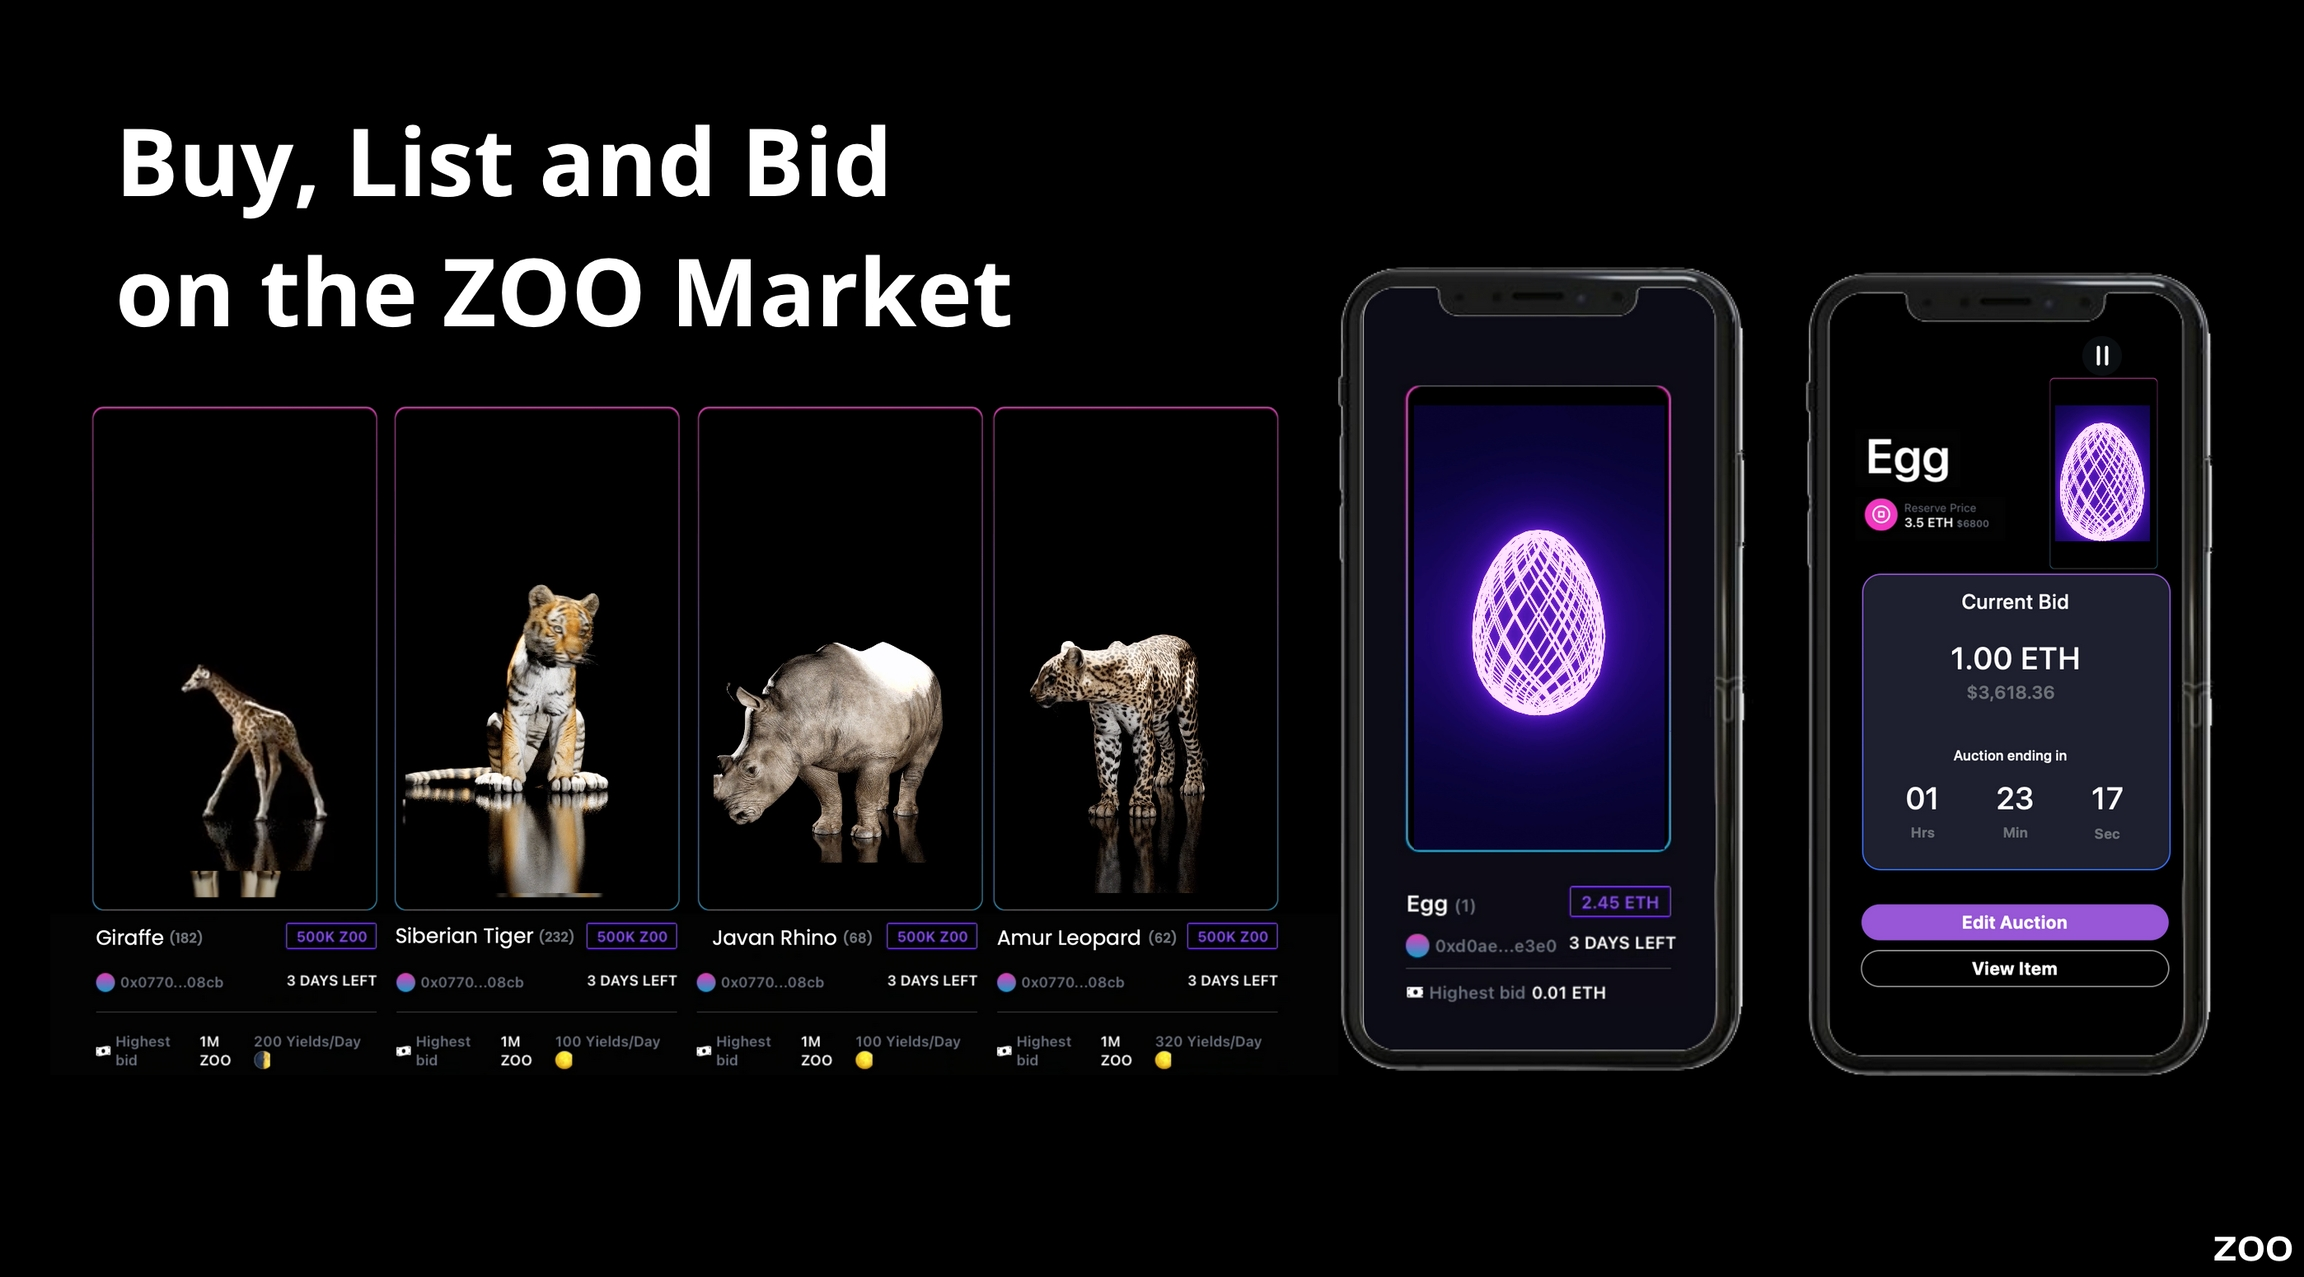
\includegraphics[width=0.85\linewidth]{figures/marketplace.png}
  \caption{Zoo Marketplace UI mockup: integrated payments (crypto and credit/debit), asset transfer, and offers/auctions.}
  \label{fig:marketplace}
\end{figure}

The Zoo Marketplace offers users the chance to purchase items using either cryptocurrency, like the \$ZOO token, or through the use of credit/debit cards directly into our marketplace. Designed with usability in mind, the Zoo team wanted to involve the most seamless checkout flow with either crypto or fiat to eliminate the most confusing terminology for newcomers in DeFi. Once a purchase is made, the seller is paid out in whatever currency they listed their NFT for, regardless of the payment method used.

Users can also use their credit/debit cards to purchase \$ZOO directly, removing one of the most prohibitive elements of the transaction process and opening up investment to many new individuals.

The marketplace also facilitates \emph{Asset Transfers}, allowing one user to transfer their NFT plus its stored value to another through a mutually agreed-upon transaction. If a user sells or trades an NFT with another user, they are also transferring the full collateral amount of the NFT.

\subsection{Leaderboard}

The Zoo leaderboard lets you compare your statistics with friends, family, and every NFT holder globally. The leaderboard also lets you make an offer bid on any NFT regardless of whether it is listed on the marketplace. Items are shown based on the NFT's total value or the user's cumulative NFT collection value.

\section{Asset Transfer}
\label{sec:asset-transfer}

\subsection{Unlocking Value via Asset Transfer Mechanisms}

As we delve deeper into the Zoo Ecosystem, it becomes clear how its dynamism offers inventive channels to realize the value of your digital companions. This section focuses on the principal methods of asset transfer in the Zoo Ecosystem --- a blend of trading NFTs on the marketplace and the unconventional practice known as \emph{burning} your NFT.

\subsubsection{Trading on the Marketplace}

A compelling means of unlocking your digital animal's value lies in its sale on the marketplace. This platform provides a stage where the inherent value of your NFT, enriched by careful nurturing and potential rarity, can be transformed into tangible returns. It is up to the seller to establish a fair selling price, preferably accounting for the accumulated value the NFT has amassed over time. Once the transaction is complete, the buyer not only inherits the animal's NFT but also the intrinsic value it has gathered, which encompasses the collateral fed to the animal and its earned rewards, potentially boosted.

The exchange is more than a mere shift of ownership; it signifies the transference of a prospering legacy. The new owner steps into a realm where they can further cultivate the NFT and harvest the rewards from their new digital ally.

\subsubsection{Burning NFTs}

Conversely, the Zoo Ecosystem introduces the concept of burning an NFT as an alternate route to tap into its value. Though the term might sound ominous, this process mirrors the real-world practice of removing a coin or note from circulation. However, this marks the end of an NFT's digital life cycle in the Zoo Ecosystem. This cessation of the NFT's lineage and its potential yield is balanced by the opportunity to promptly access the NFT's underlying earned value.

These mechanisms of trading or burning NFTs are instrumental in fostering a dynamic and vibrant Zoo Ecosystem. They ensure high liquidity, contribute to maintaining high value for NFTs based on their underlying assets, and enhance their inherent worth.

\section{Gameplay Functions}
\label{sec:gameplay-fn}

\subsection{Pre-Drop Whitelist}

The Zoo experience begins with our NFT eggs and an NFT egg drop. Each Zoo NFT egg drop features a series of animals from egg, to juvenile, adolescent, and mature forms. Drops may be themed based upon something related to the natural world, a cultural celebration, current events, partnerships and licensing agreements, or any number of other potential sources of inspiration. Before each NFT egg drop, new or existing users have the opportunity to purchase one random NFT egg --- of potentially any available rarity tier --- for the price of the most common egg. When the NFT eggs are distributed to the presale purchasers, their egg type and its related value are revealed. Some lucky users will end up with our rarest and most valuable NFT egg for the price of our lowest-cost and most common one.

\subsection{Original Egg Price}

The original price of the three varieties of eggs determines the cost to mint the future animals. The original prices are:
\begin{itemize}
  \item \textbf{Sublime Egg} --- most rare, 5\% of distribution: 1 ETH.
  \item \textbf{Rare Egg} --- second most rare, 15\% of distribution: 0.5 ETH.
  \item \textbf{Endangered Egg} --- most common, 85\% of distribution: 0.1 ETH.
\end{itemize}

Once a user has purchased their NFT egg and it resides in their wallet, they may choose to hatch their egg into a baby NFT animal. To mint the teen version, the user must feed the NFT 1$\times$ the original egg price. When doing this, the user is not spending those tokens; they are staking them into the NFT.

After their NFT animal has hatched and they have had the chance to experience it in its teen form, the user can choose to feed the NFT's original base price 2$\times$ to make their NFT animal grow into adult form, minting another NFT. Now they have collateral in the adult NFT worth 2$\times$ the original egg price. They can find another adult of the same species and breed them to mint a new egg of the same rarity by paying the breeding fee, which is 3$\times$ the price of the original egg.

From this point forward, the user can continue to feed their NFT animal crypto --- both \$ZOO and virtually any other cryptocurrency --- to stake the tokens into the NFT animal's liquidity pool, which results in the boosts described in Section~\ref{sec:collateral}.

\section{Gen 0 NFT Drop}
\label{sec:gen0}

\textit{Zoo Labs introduces an enhanced reward system with unique daily rewards to engage and reward the Zoo community, fostering a sustainable and democratic ecosystem governed by the Zoo DAO.}

In our highly anticipated Gen 0 NFT drop, we introduce an enhanced reward system that aims to create an engaging and rewarding experience for our Zoo community. Each Gen 0 animal NFT comes with its own unique set of daily rewards, designed to incentivize active participation and offer ongoing benefits. Whether it is additional \$ZOO tokens, exclusive NFTs, or other in-game rewards, our daily rewards system ensures that there is always something to look forward to.

Boosts have a direct impact on the daily rewards. By adding collateral to the animals they own (\emph{Feeding}), players boost their daily rewards. These boosts amplify the potential rewards earned, providing additional incentive for collectors to enhance the value of their animals over time.

The initial rewards are carved out during the Gen 0 NFT drop, with 50\% of the entire token supply allocated towards rewards. This allocation sets the foundation for a robust and sustainable reward system. Any further rewards, reward modifications, or duration changes are subject to the decisions made by the Zoo DAO. The daily rewards for each Gen 0 animal have a finite duration: rewards continue for two years after the animal is minted.

\subsection{Breeding and Hatching: A Brief Guide}

In Zoo Labs' ecosystem, breeding requires two adult NFT animals of the same species but can be of any generation. The cost of breeding is determined by the original egg price (OEP), which varies based on the rarity of the animal. A Sublime egg costs 1 ETH; a Rare egg costs 0.5 ETH; an Endangered egg costs 0.05 ETH.

Upon successful breeding, an egg is minted and can be hatched for free or sold on the marketplace. Hatching yields a baby animal that can be grown into a teen by locking in collateral (the feeding action). To advance a baby to teen, lock in collateral equal to the OEP. Transforming a teen into an adult requires collateral equivalent to 2$\times$ OEP. Breeding fees of 3$\times$ OEP are directed to the DAO rather than staking collateral.

\subsection{Generational Limits}

Each egg generation has a limit of one baby, one teen, and one adult that can be minted. Adults with breeding privileges can breed with another adult of the same species to mint a subsequent egg generation. Restrictions on the number of generations from the initial drop:
\begin{itemize}
  \item Generation 1: 7 breeding allowances.
  \item Generation 2: 6 allowances.
  \item Generation 3: 5 allowances.
  \item Generation 4: 4 allowances.
  \item Generation 5: 3 allowances.
  \item Generation 6: 2 allowances.
  \item Generation 7: 0 allowances.
\end{itemize}

Adult animals can be sold with or without remaining breeding privileges. If a first-generation animal is bred only twice and burned after 20 days, no further offspring can be produced from that animal.

\subsection{Daily Allowances by Rarity}

\begin{itemize}
  \item \textbf{Sublime Animals}: Baby --- 1 \$ZOO; Teen --- 2 \$ZOO; Adult --- 3 \$ZOO.
  \item \textbf{Rare Animals}: Baby --- 0.25 \$ZOO; Teen --- 0.5 \$ZOO; Adult --- 1 \$ZOO.
  \item \textbf{Endangered Animals}: Baby --- 0.05 \$ZOO; Teen --- 0.1 \$ZOO; Adult --- 0.2 \$ZOO.
\end{itemize}
